
The proposed ECal trigger was simulated to test trigger cuts, verify that the trigger has acceptable efficiency for A' events, and verify that the trigger rate is compatible with the HPS DAQ in all running conditions.

Trigger simulation is done in three stages. 
First, various packages are used to simulate beam interactions in the target---details are given in Section \ref{sec:backgrounds}.
The beam background files (equivalent to 100 ms of beam at each energy) are merged into a common StdHep format such that each event corresponds to one 2 ns bunch of the beam at the planned beam current.
A' tridents are also simulated using MadGraph. 
Next, the Geant4-based simulations system SLIC \cite{slic} is used to simulate interactions and energy deposition in the magnetic field, tracker, vacuum chamber and ECal. 
Finally, readout and trigger simulation is done using LCSim. The simulation takes time-dependent effects such as pileup into account; pulse shapes, trigger state, etc. are updated at 2 ns intervals corresponding to the bunch frequency.
This is a faithful simulation of the detector, DAQ and trigger and has been tested against the actual performance of the test run detector and DAQ. See Section \ref{sec:triggerdaq} for details of the readout, clustering and trigger algorithms.

The trigger parameters described in Section \ref{sec:triggerdaq} are chosen by running the simulation and plotting the relevant variables for beam background and A' events. 
This is done for each beam energy and a set of A' masses for each beam energy. Examples of these comparisons are shown in Figures \ref{fig:coplanarity}, \ref{fig:energy-distance} and \ref{fig:ediff}.

\begin{figure}[ht]
	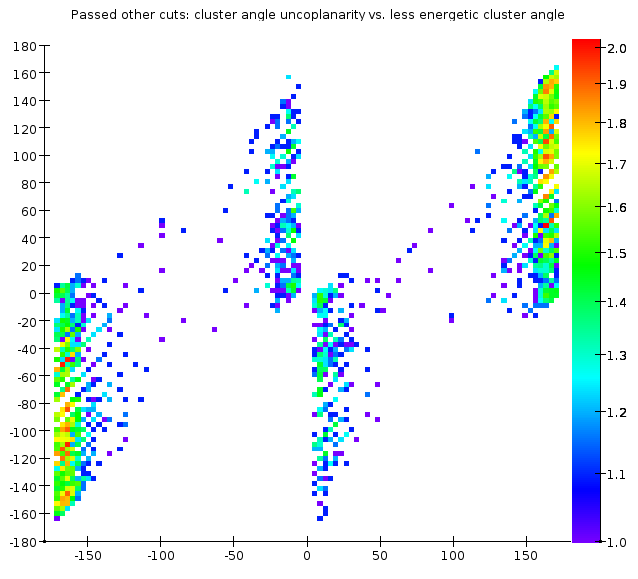
\includegraphics[width=0.4\textwidth]{performance/trigger/coplanarity_22}
	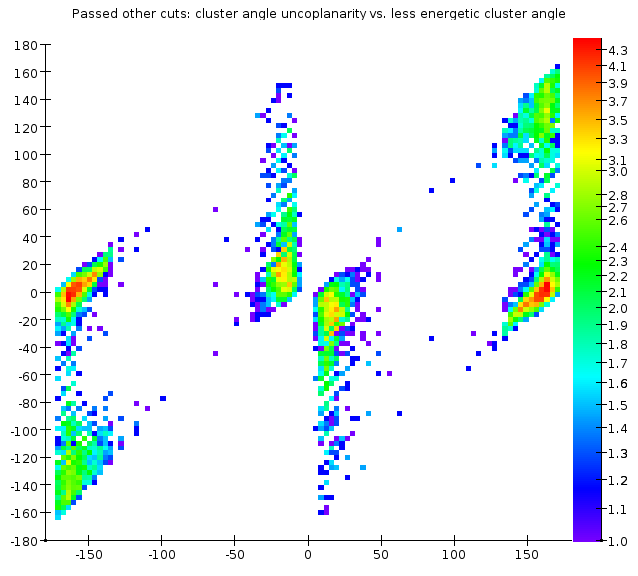
\includegraphics[width=0.4\textwidth]{performance/trigger/coplanarity_22_075mev}
	\caption{\small{Deviation of cluster pairs from coplanarity (units of degrees) for 2.2 GeV beam; background and 75 MeV A' tridents are shown.}}
	\label{fig:coplanarity}
\end{figure}

\begin{figure}[ht]
	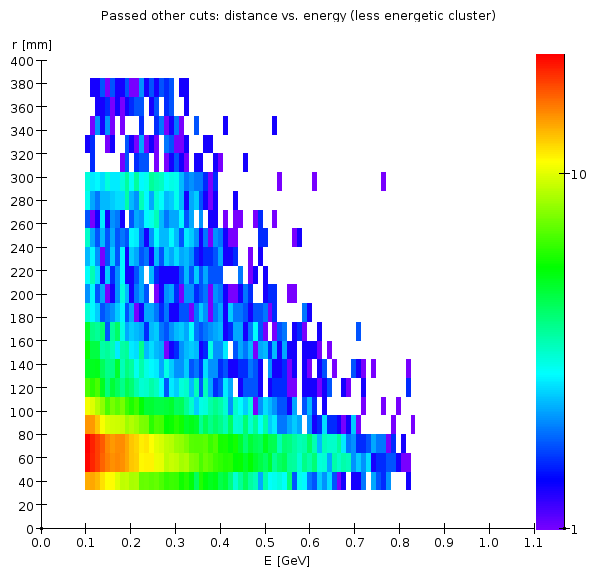
\includegraphics[width=0.4\textwidth]{performance/trigger/energy-distance_22}
	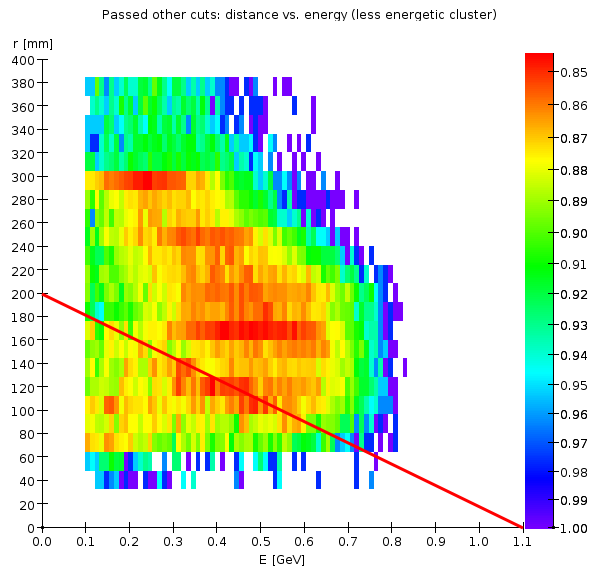
\includegraphics[width=0.4\textwidth]{performance/trigger/energy-distance_22_075mev}
	\caption{\small{Energy and distance from beam axis of the lower-energy cluster, for 2.2 GeV beam; background and 75 MeV A' tridents are shown.}}
	\label{fig:energy-distance}
\end{figure}

\begin{figure}[ht]
	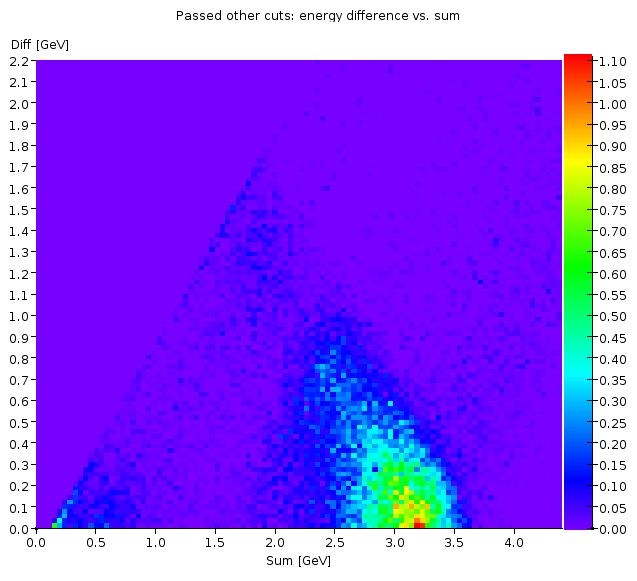
\includegraphics[width=0.4\textwidth]{performance/trigger/ediff_22}
	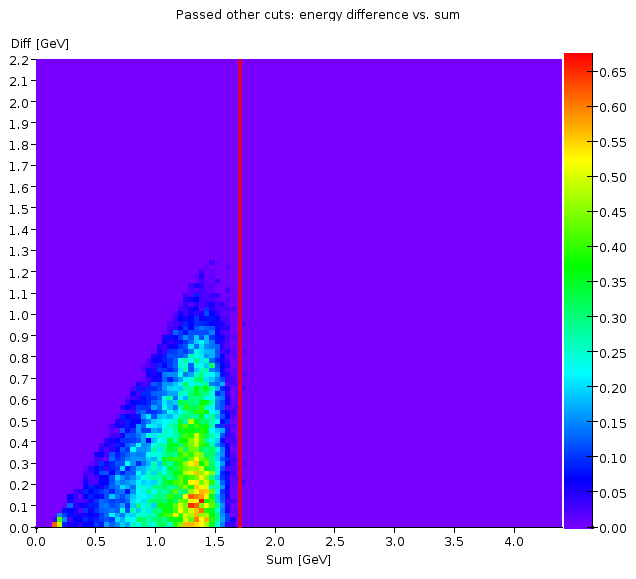
\includegraphics[width=0.4\textwidth]{performance/trigger/ediff_22_075mev}
	\caption{\small{Energy sum and difference of cluster pairs, for 2.2 GeV beam; background and 75 MeV A' tridents are shown.}}
	\label{fig:ediff}
\end{figure}

The following trigger parameters were determined to be independent of beam energy:
\begin{itemize}
	\item Minimum cluster energy ($E_{min}$): 0.1 GeV
	\item Energy-distance distance ($r_{edist}$): 200 mm
	\item Energy-distance energy ($E_{edist}$): $0.5\times E_{beam}$
\end{itemize}

The remaining trigger parameters given in Section \ref{sec:triggerdaq} do not have a significant effect on specificity of the trigger.

\begin{table}
	\begin{tabular}{|l|r|r|r|}
		\hline
		Beam energy [GeV] & $E_{max}$ [GeV] & $Esum_{max}$ [GeV] & $\Delta\phi_{max}$ [$^\circ$] \\
		\hline
		1.1	&	0.7	&	0.8	&	90\\
		2.2	&	1.6	&	1.7	&	45\\
		6.6	&	5.0	&	5.5	&	60\\
		\hline
	\end{tabular}
	\caption{ {\small Trigger parameters optimized for different beam energies.}
	\label{tab:trigcuts}}
\end{table}

Trigger efficiency for A' events is defined as the fraction of A' tridents (generated without fiducial cuts) that produce a trigger.

Trigger rates are shown in Table \ref{tab:trigrates}. These rates are safely under the maximum readout rate of 43 kHz set by the SVT. 
The addition of pions to the 6.6 GeV background sample does not have a significant effect on the trigger rate.

\begin{table}
	\begin{tabular}{|l|r|}
		\hline
		Sample &  Rate (kHz)\\
		\hline
		1.1 GeV	EGS5 				& 15.7 $\pm$ 0.4	\\
		1.1 GeV EGS5+tridents			& 17.6 $\pm$ 0.6	\\
		2.2 GeV	EGS5 				& 11.2 $\pm$ 0.3	\\
		2.2 GeV EGS5+tridents			& 15.8 $\pm$ 0.4	\\
		6.6 GeV	EGS5 				& 10.2 $\pm$ 0.3	\\
		6.6 GeV EGS5+tridents			& 12.6 $\pm$ 0.4	\\
		%6.6 GeV EGS5+tridents+pions (FLUKA)	& 7.3 $\pm$ 0.3	\\
		%6.6 GeV EGS5+tridents+pions (G4)	& 7.0 $\pm$ 0.3	\\
		\hline
	\end{tabular}
	\caption{ {\small Trigger rates using various background samples. }
	\label{tab:trigrates}}
\end{table}

Trigger efficiency for A' events is defined as the fraction of A' tridents (generated without fiducial cuts) that produce a trigger.

For the performance of the experiment, we are interested in the combined efficiency of the trigger and tracker: the fraction of A' tridents that produce a trigger and leave enough hits in the tracker for a pair of tracks to be reconstructed.
We simulate charge deposition and readout of the tracker (turning off the generation of noise hits), and check each sensor for hits. 
If the DAQ reads out hits in four stereo pairs in each half of the tracker, the event is in the combined acceptance.

Both efficiency values (trigger only, and combined) are shown in Figure \ref{fig:trigeff}. 
Both trigger and tracker acceptances are dominated by the geometric acceptances of the ECal and tracker.

\begin{figure}[ht]
	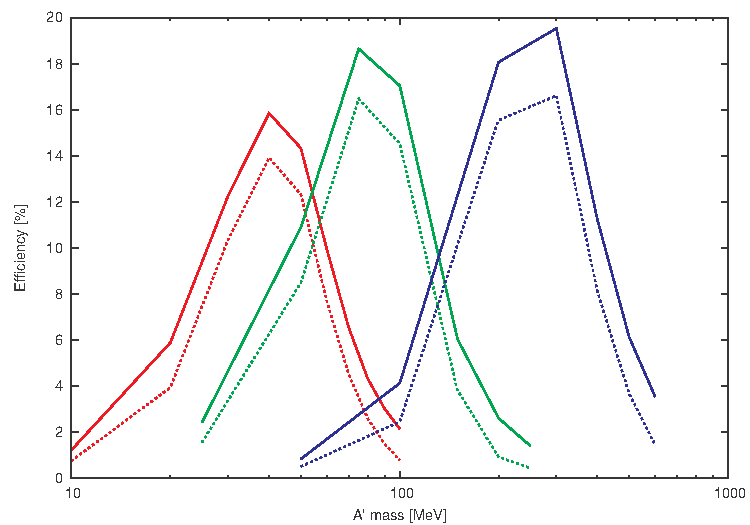
\includegraphics[width=\textwidth]{performance/trigger/ap_eff}
	\caption{\small{Trigger efficiency (solid lines) and combined efficiency (dashed lines) as a function of A' mass, at beam energies of 1.1, 2.2 and 6.6 GeV (red, green and blue respectively).}}
	\label{fig:trigeff}
\end{figure}

